\apendice{Documentación de usuario}

\section{Introducción}
En este anexo se describirá el proceso que deben seguir los usuarios para la correcta utilización XacoMeterII.
\section{Requisitos de usuarios}
Se puede acceder a la aplicación XacoMeterII a través del enlace \url{https://tfg-nataliafranco-xacometer2.herokuapp.com/}.\\
La página ha sido desplegada a través de Heroku, pero debido a sus limitaciones de tiempo de espera y a las restricciones de la API de Twitter en cuanto a recopilación de datos, el modo \textit{Administrador} solo estará disponible para su uso en modo local. En caso de intentar acceder como administrador en la aplicación desplegada y solicitar crear la base de datos o actualizarla, la propia página generará un \textit{'timeout'}.\\
Para poder utilizar todas las funciones, incluyendo el modo \textit{'Administrador'}, se facilita una máquina virtual con todos los recursos instalados y puesta en marcha para funcionar en su totalidad, de esta manera no se tendrán limitaciones, excepto las marcadas por la API de Twitter.\\
Al ser una aplicación web se requiere acceso a internet y un navegador, o en el caso de utilizar el modo \textit{Administrador}, se requiere de la descarga de la máquina virtual.
\section{Instalación}
Los usuarios no necesitan instalar nada en el equipo para el uso de XacoMeterII, ya que se accede con un navegador web a través de internet.\\
En el caso de utilizar el modo \textit{'Administrador'} se dispone de una máquina virtual.

\section{Manual del usuario}
A continuación, se detallan los pasos a seguir para el correcto uso de la aplicación.
\subsection{Inicio}
Para iniciar la aplicación se accede a \url{https://tfg-nataliafranco-xacometer2.herokuapp.com/} en un navegador web.
Una vez se accede a la página web, lo primero que se visualiza es una página de inicio, en la que se puede ver un mapa dinámico con los Bienes de Interés Cultural del Camino de Santiago Francés en Castilla y León situados en él, una barra navegadora y un desplegable con el nombre de los BICs (Figura E.1).\\
\begin{figure}[h!]
    \centering
    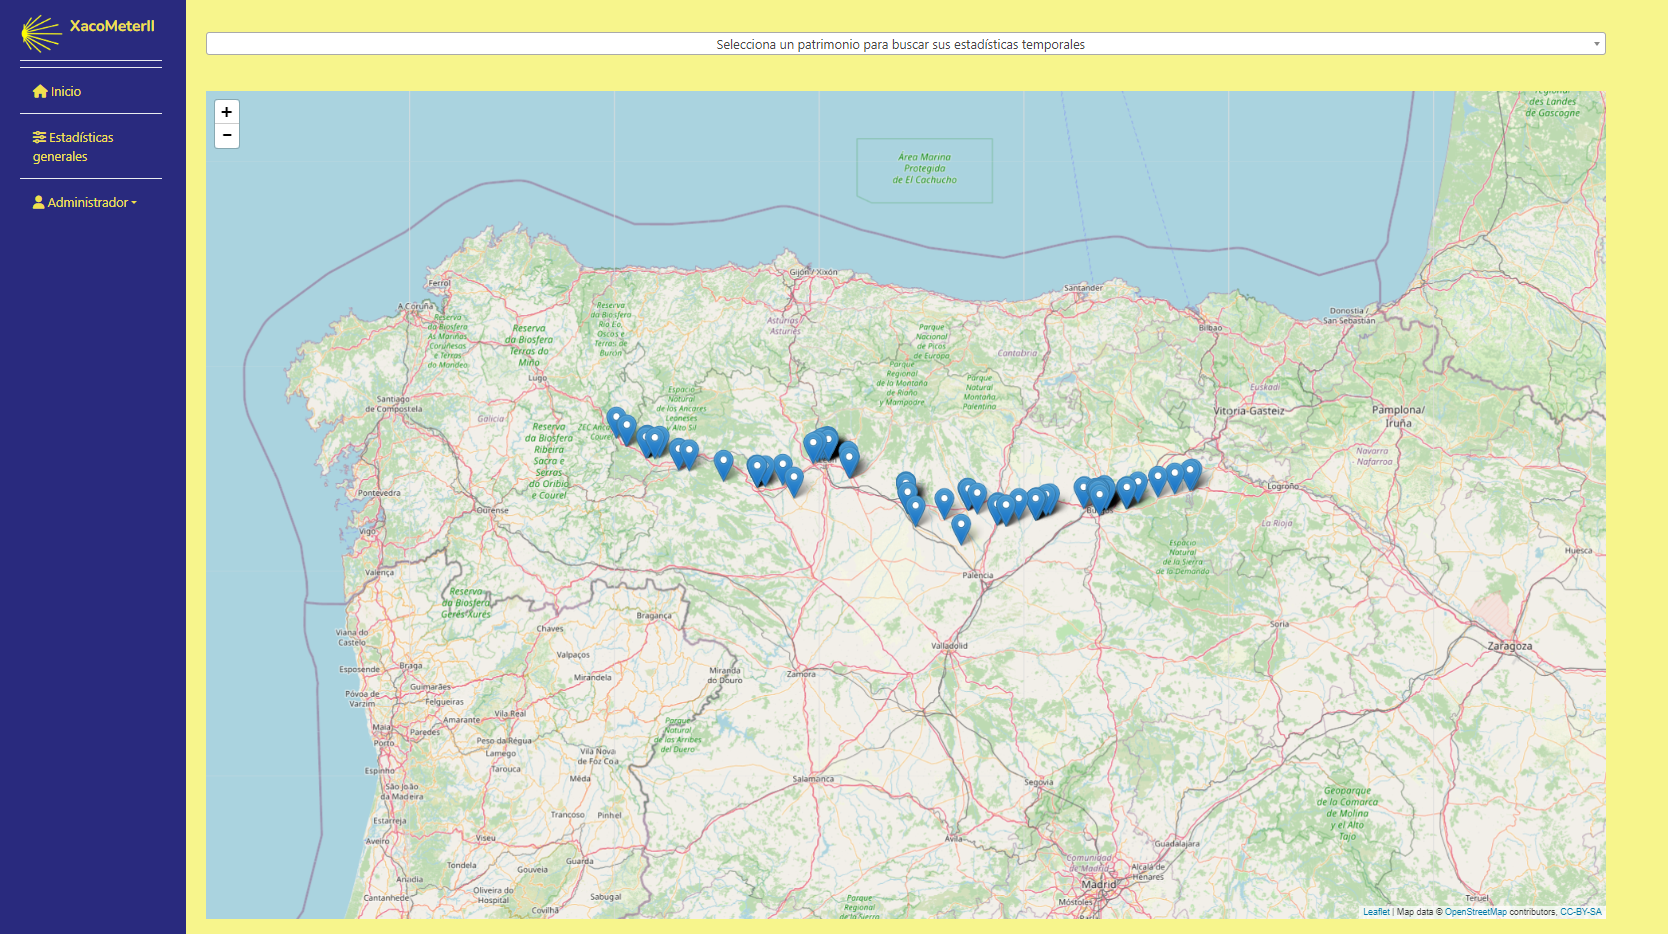
\includegraphics[scale=0.3]{img/Inicio.png} \\
    \caption{Documentación de usuario - Inicio}
    \label{Documentación de usuario - Inicio}
\end{figure}
\subsection{Barra navegadora}
Este elemento va a estar disponible en todas las páginas de la aplicación y va a permitir realizar las diferentes acciones posibles (Figura E.2, Figura E.3).\\
Además, se divide en dos secciones, según los permisos del usuario.\\
El botón \textbf{INICIO}, será un botón que puedan acceder todos los usuarios, con el que se redireccionará al usuario a la página de inicio.\\
El botón \textbf{ESTADÍSTICAS GENERALES}, será un botón que puedan acceder todos los usuarios, con el que se redireccionará al usuario a la página de estadísticas generales de todos los BICs.\\
El botón \textbf{ADMINISTRADOR} solo estará disponible para los usuarios en modo administrador y se podrá acceder tanto al inicio de sesión como a las opciones de administrador y además, permitirá cerrar sesión, todo ello contando con que el usuario ha introducido las credenciales correctamente.

\begin{figure}[H]
    \begin{minipage}[b]{0.5\linewidth}
        \centering
        
\includegraphics[scale=0.7]{img/BarraComprimida.png} \\
        \caption{Documentación de usuario - Barra de navegación comprimida}
        \label{Documentación de usuario - Barra de navegación comprimida}
    \end{minipage}
    \hspace{0.5cm}
    \begin{minipage}[b]{0.5\linewidth}
        \centering
        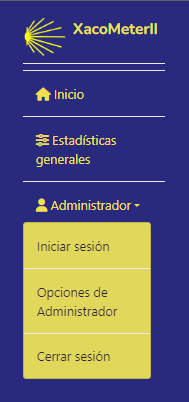
\includegraphics[scale=0.7]{BarraDesplegada.png}
        \caption{Documentación de usuario - Barra de navegación desplegada}
        \label{Documentación de usuario - Barra de navegación desplegada}
    \end{minipage}
\end{figure}

\subsection{Selección del patrimonio}
En la ventana de inicio se puede seleccionar un BIC para ser redirigido a la página de estadísticas temporales del mismo.\\
Esto se puede realizar de dos maneras:
\begin{enumerate}
    \item Utilizando el mapa dinámico (Figura E.4), con el que el usuario puede moverse con el ratón y seleccionar el BIC que desee.
    \begin{figure}[h!]
        \centering
        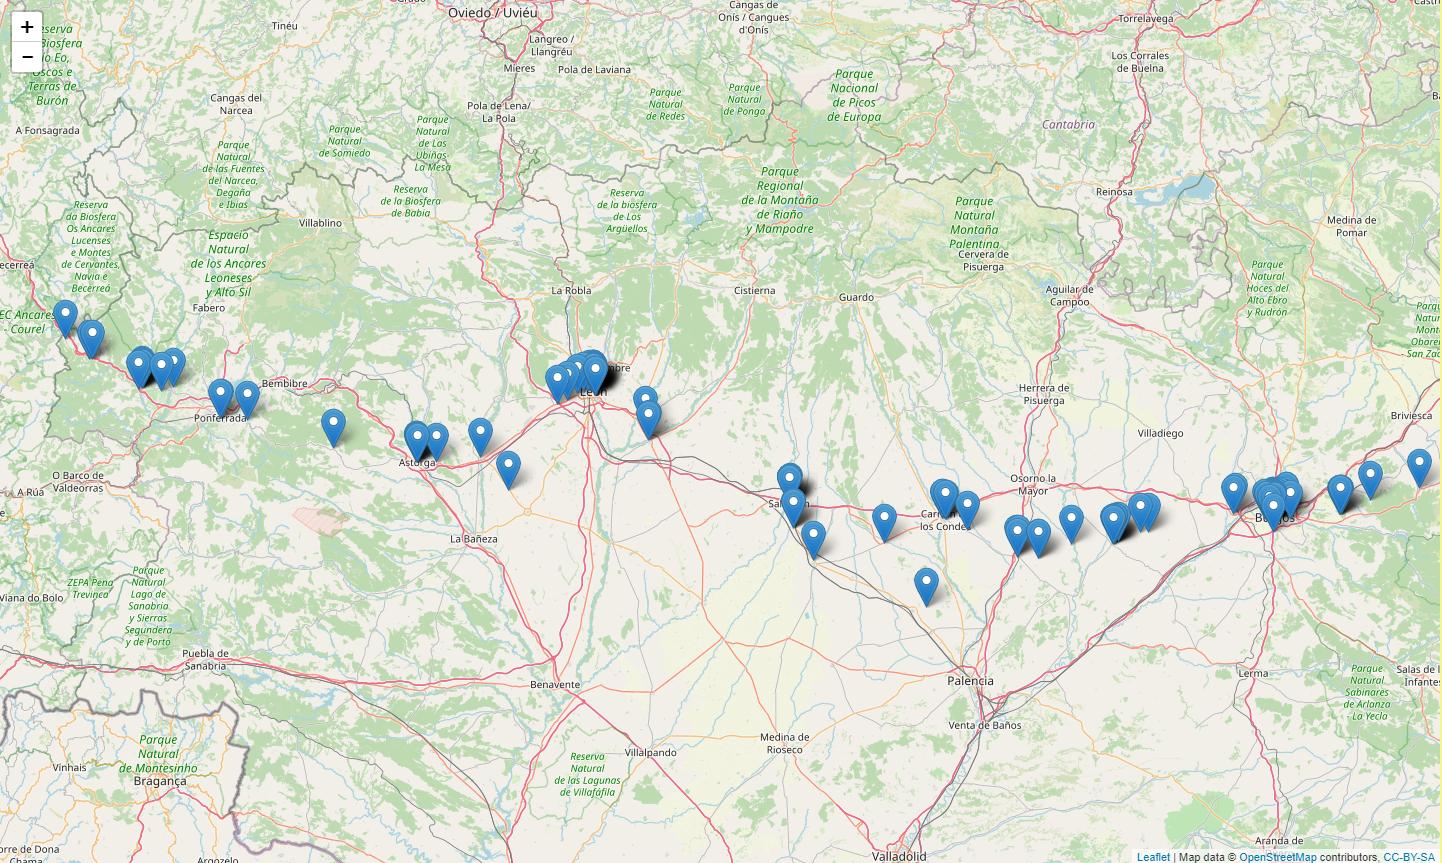
\includegraphics[scale=0.3]{img/Mapa.png} \\
        \caption{Documentación de usuario - Mapa}
        \label{Documentación de usuario - Mapa}
    \end{figure}
    \item Abriendo el desplegable que está situado encima del mapa y seleccionando un BIC (Figura E.5).
    \begin{figure}[h!]
        \centering
        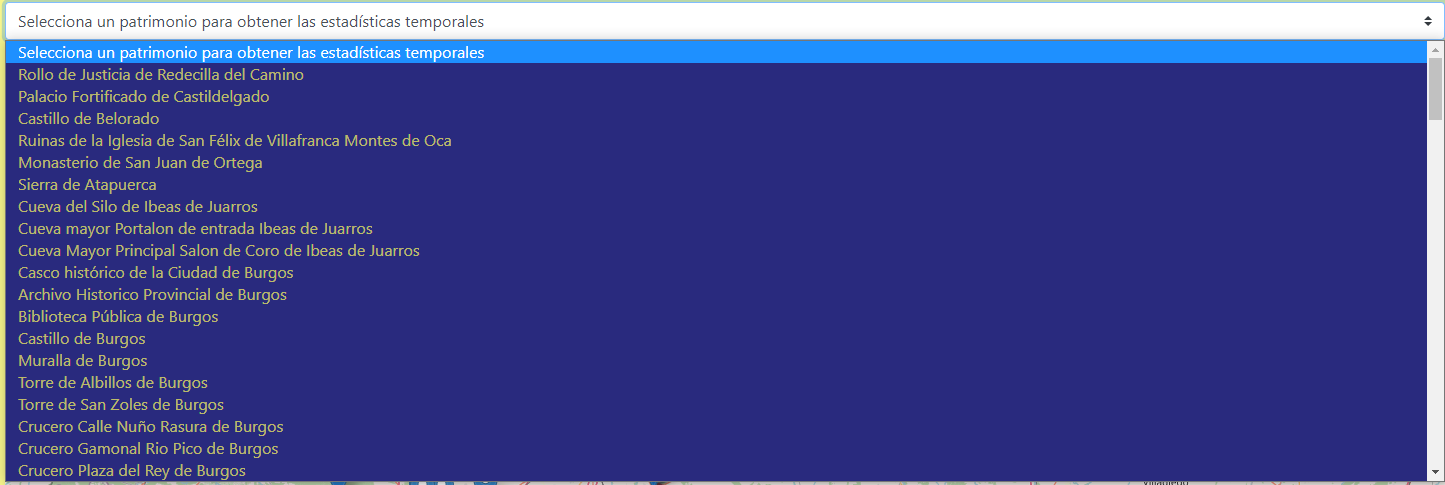
\includegraphics[scale=0.3]{img/DesplegablePatrimonios.png} \\
        \caption{Documentación de usuario - Desplegable patrimonios}
        \label{Documentación de usuario - Desplegable patrimonios}
    \end{figure}
\end{enumerate}
\subsection{Página de estadísticas temporales}
Una vez se ha seleccionado un BIC en la página de inicio, se redireccionará al usuario a la página de estadísticas temporales, en la que se mostrarán las estadísticas temporales del BIC entre las fechas existentes en la base de datos y el análisis de sentimientos (Figura E.6).\\
Esta página permite modificar las fechas de inicio y fin de las estadísticas, teniendo en cuenta que la fecha de inicio debe ser anterior que la fecha de fin.
Además esta página permite volver a la página de inicio y descargar el csv con los datos del patrimonio.
\begin{figure}[h!]
    \centering
    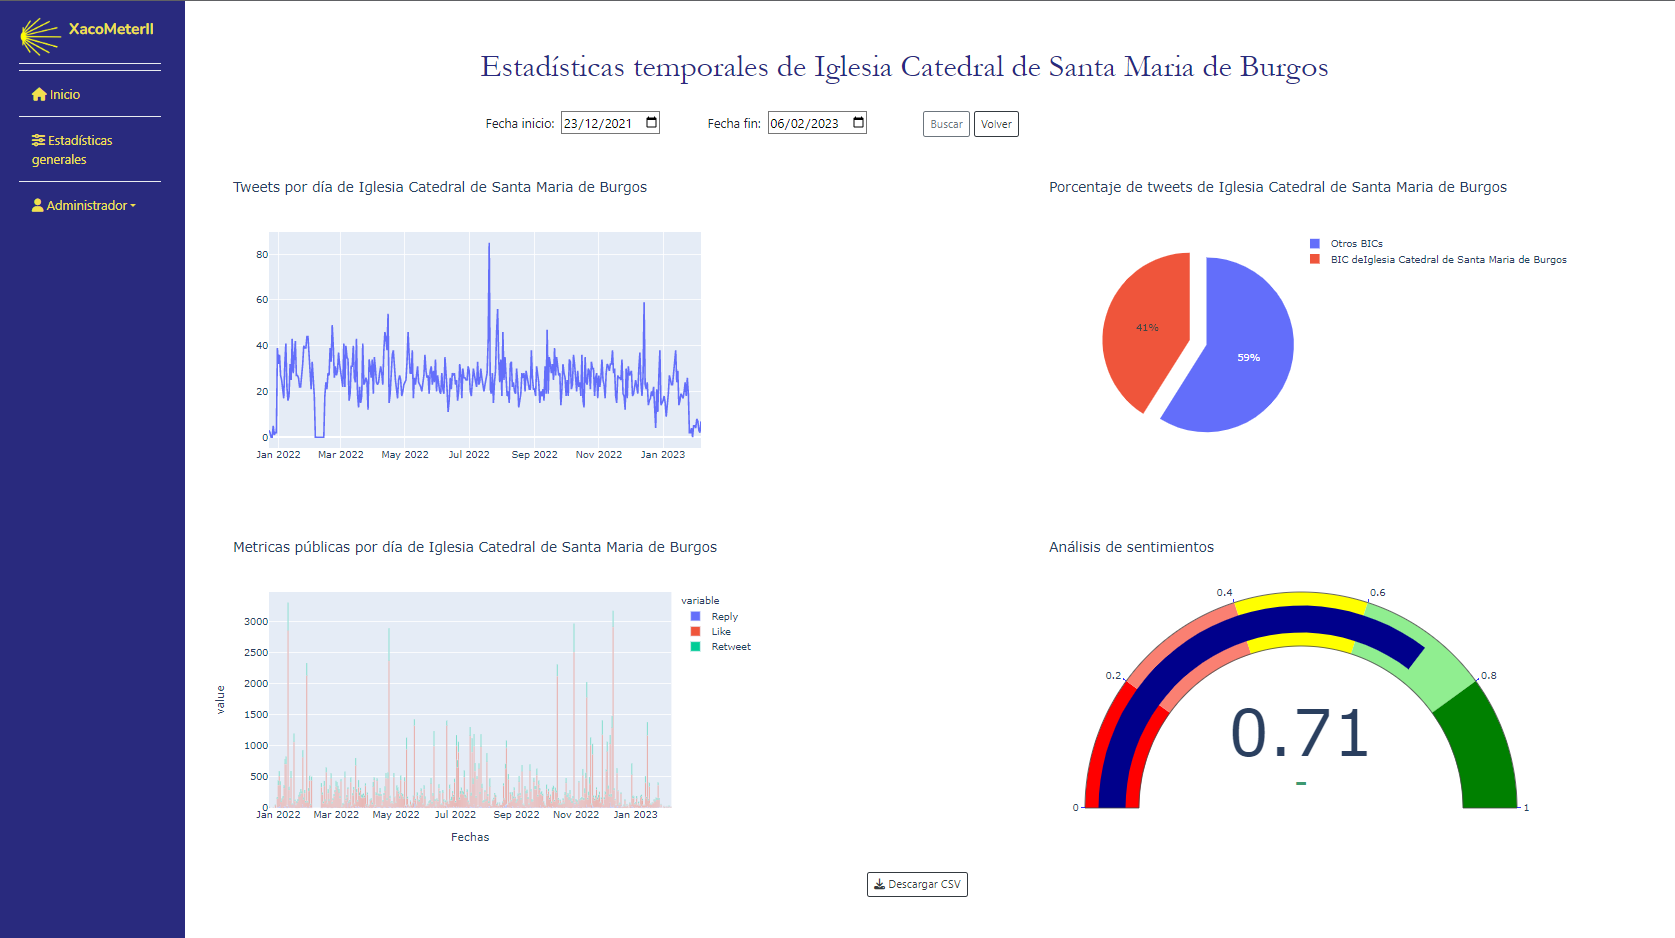
\includegraphics[scale=0.25]{img/Mejoras.png} 
    \caption{Documentación de usuario - Estadísticas temporales}
    \label{Documentación de usuario - Estadísticas temporales}
\end{figure}
\subsection{Gráfico de tweets por día}
Es el primer gráfico que se muestra en la página de estadísticas temporales. Muestra los tweets que se diariamente de este BIC en el periodo de tiempo establecido (Figura E.7).\\
Este gráfico es dinámico y se puede descargar en formato \textit{.PNG}, así como también se puede mover, ampliar y visualizar los datos de cada uno de sus puntos al poner el ratón sobre ellos.
\begin{figure}[h!]
    \centering
    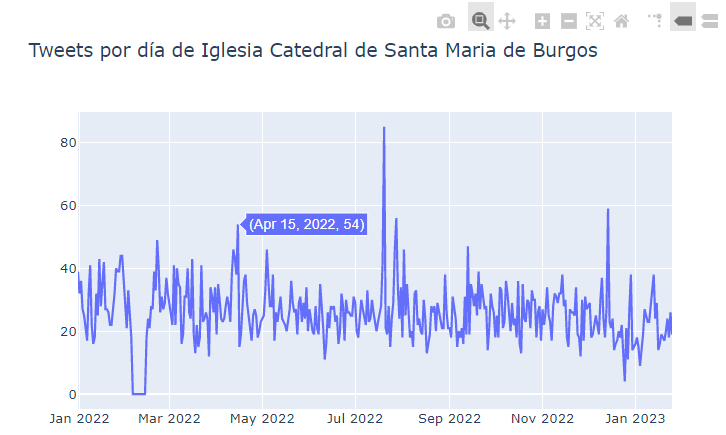
\includegraphics[scale=0.4]{img/TweetsDia.png} \\
    \caption{Documentación de usuario - Gráfico de tweets por día}
    \label{Documentación de usuario - Gráfico de tweets por día}
\end{figure}
\subsection{Gráfico de porcentaje de tweets}
En el segundo gráfico que se muestra en la página de estadísticas temporales, se puede ver el diagrama circular que muestra el porcentaje de tweets del BIC en cuestión con respecto al total de tweets (Figura E.8).\\
Este gráfico permite saber cuántos tweets totales tiene cada uno de los sectores poniendo el ratón sobre cada uno de ellos. También es posible descargar el gráfico en formato \textbf{.PNG}.\\
\begin{figure}[h!]
    \centering
    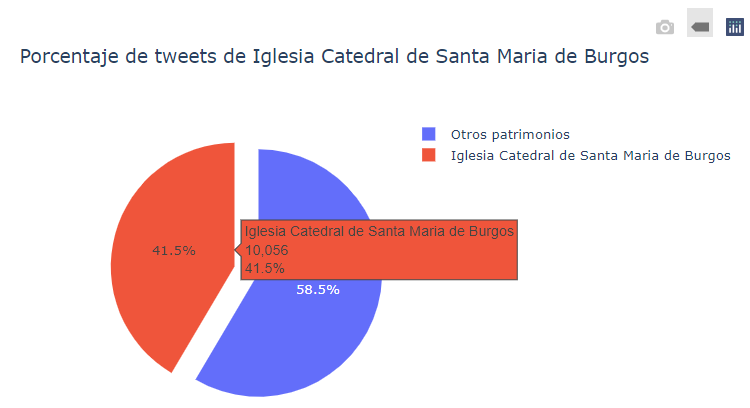
\includegraphics[scale=0.35]{img/TweetsPorcentaje.png} \\
    \caption{Documentación de usuario - Gráfico de porcentaje de tweets}
    \label{Documentación de usuario - Gráfico de porcentaje de tweets}
\end{figure}
\subsection{Gráfico de métricas públicas}
En el gráfico inferior de la página de estadísticas temporales, se pueden comparar las métricas públicas de cada BIC en el periodo temporal seleccionado. En este gráfico se utilizan los parámetros de \textit{likes, retweets y replies} que han tenido en un día los tweets publicados sobre ese BIC (Figura E.9).\\
Este gráfico permite realizar las mismas acciones que el gráfico de tweets por día, añadiendo la opción de seleccionar libremente un conjunto de datos del gráfico.
\begin{figure}[h!]
    \centering
    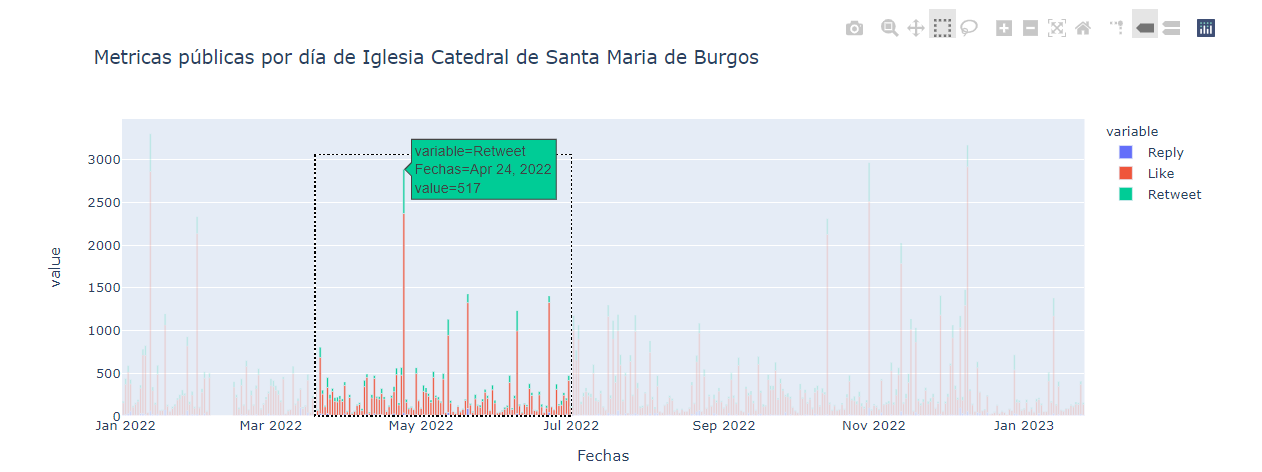
\includegraphics[scale=0.3]{img/MetricasPublicas.png} \\
    \caption{Documentación de usuario - Gráfico de métricas públicas}
    \label{Documentación de usuario - Gráfico de métricas públicas}
\end{figure}


\subsection{Gráfico de análisis de sentimientos}
En el cuarto gráfico de la página de estadísticas temporales se muestra en un diagrama semicircular del 0 (negativo) al 1 (positivo) el índice medio de sentimiento de los tweets del BIC seleccionado en el periodo temporal elegido (Figura E.10). \\
Este gráfico también muestra el número exacto del índice medio de sentimiento obtenido del BIC entre las fechas seleccionadas.\\
\begin{figure}[h!]
    \centering
    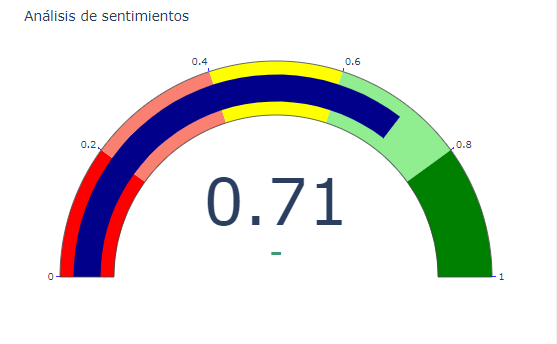
\includegraphics[scale=0.5]{img/AnalisisSentimientos.png} \\
    \caption{Documentación de usuario - Análisis de sentimientos}
    \label{Documentación de usuario - Análisis de sentimientos}
\end{figure}
\subsection{Descarga de datos}
Además, en la página de estadísticas temporales, se incluye un botón (Figura E.11) que, al pulsar en él, descarga un fichero \textit{.csv} (Figura E.12), que puede ser importado a Excel, en el que se muestran todos los tweets con sus parámetros por columnas.
\begin{figure}[H]
    \begin{minipage}[b]{0.5\linewidth}
        \centering
        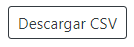
\includegraphics[scale=0.6]{img/Descarga.png} 
        \caption{Documentación de usuario - Botón descargar}
        \label{Documentación de usuario - Botón descargar}
    \end{minipage}
    \hspace{0.4cm}
    \begin{minipage}[b]{0.5\linewidth}
        \centering
        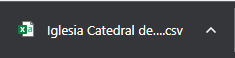
\includegraphics[scale=0.55]{Descargacsv.png}
        \caption{Documentación de usuario - Descarga de .csv}
        \label{Documentación de usuario - Descarga de .csv}
    \end{minipage}
\end{figure}
La visualización de los datos puede realizarse de la siguiente manera:\\
\begin{enumerate}
    \item Entrar en Excel.
    \item Crear una hoja en blanco.
    \item Ir a la pestaña de datos y pulsar sobre \textbf{importar csv}.
    \item Se abrirá una pestaña con las opciones del csv (Figura E.13).
    \begin{figure}[h!]
        \centering
        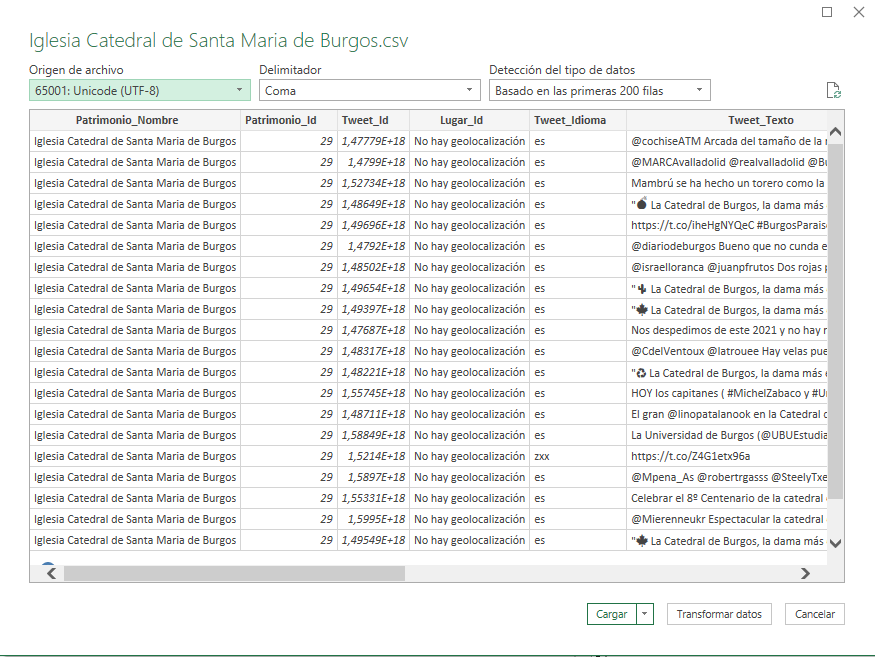
\includegraphics[scale=0.45]{img/ProcesoExcel.png} \\
        \caption{Documentación de usuario - Importar csv}
        \label{Documentación de usuario - Importar csv}
\end{figure}
    \item Dar al botón \textbf{cargar} (Figura E.14).
\end{enumerate}
\begin{figure}[h!]
    \centering
    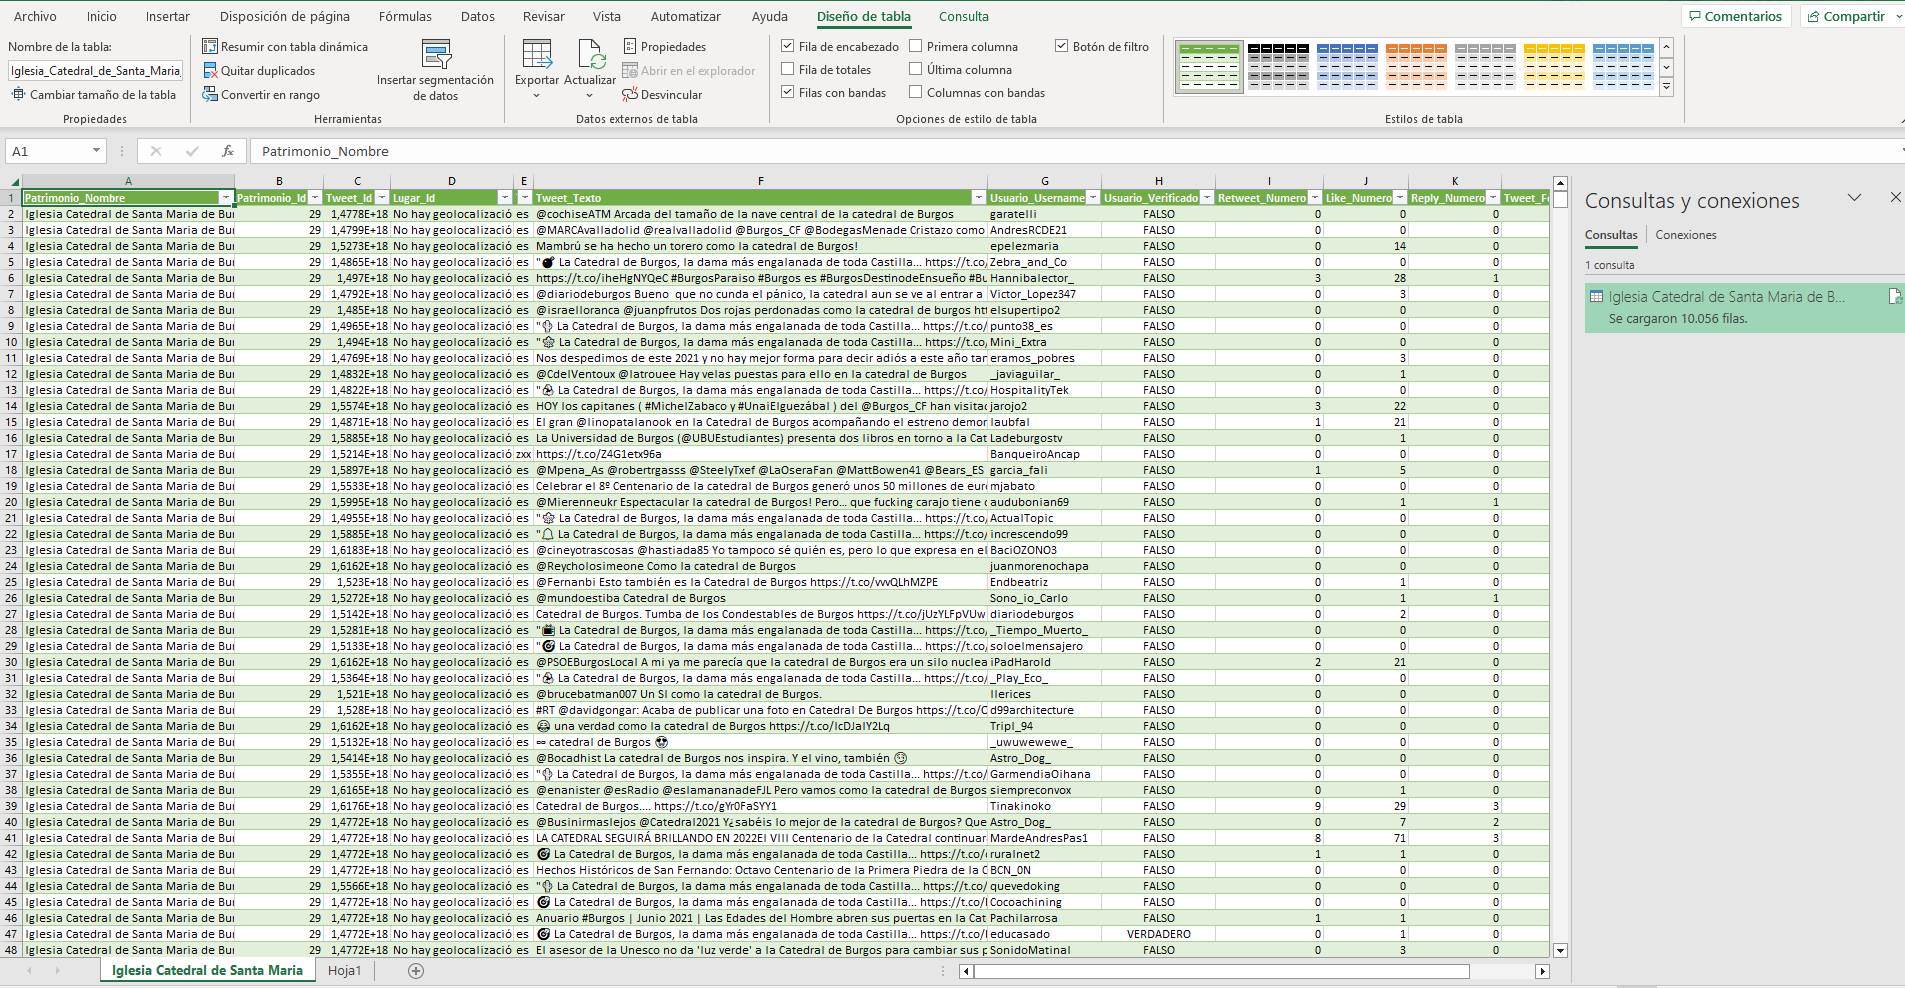
\includegraphics[scale=0.2]{img/Excel.png} \\
    \caption{Documentación de usuario - Visualización en Excel}
    \label{Documentación de usuario - Visualización en Excel}
\end{figure}
\subsection{Página de estadísticas temporales}
Una vez se ha pulsado en la barra navegadora el botón 'Estadísticas generales', se redireccionará al usuario a la página de estadísticas generales, en la que se mostrarán el total de tweets de todos los BIC entre las fechas existentes en la base de datos (Figura E.15).\\
Esta página permite modificar las fechas de inicio y fin de las estadísticas, teniendo en cuenta que la fecha de inicio debe ser anterior que la fecha de fin.
Además esta página permite volver a la página de inicio.
\begin{figure}[h!]
    \centering
    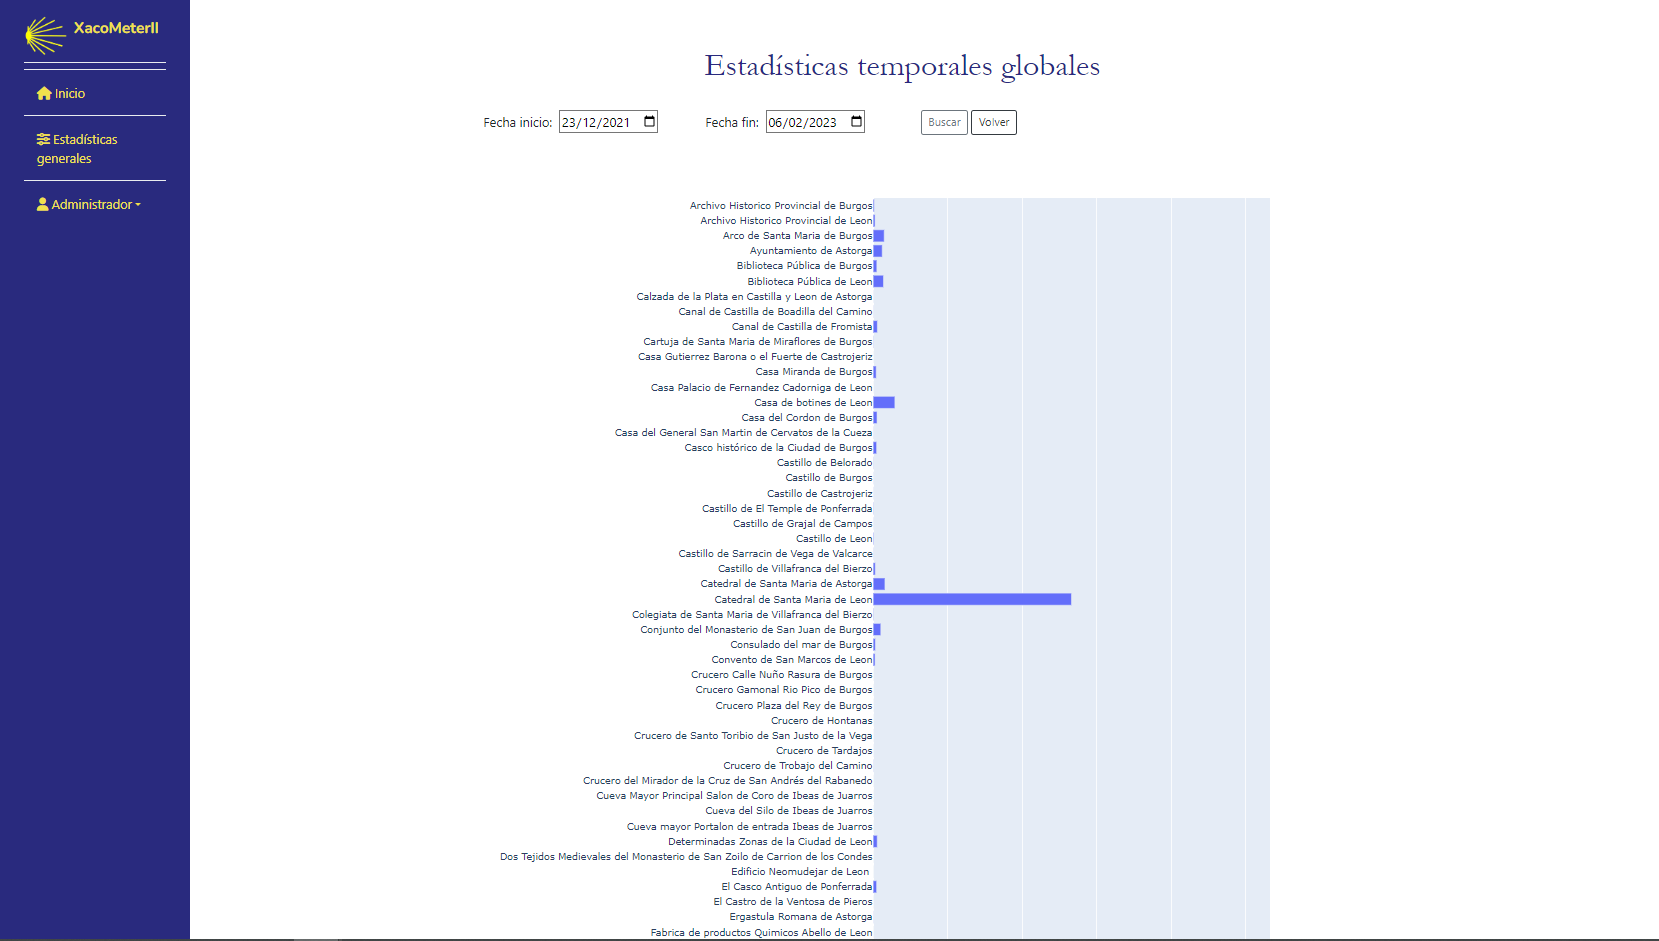
\includegraphics[scale=0.3]{img/EstadisticasGenerales.png} 
    \caption{Documentación de usuario - Estadísticas generales}
    \label{Documentación de usuario - Estadísticas generales}
\end{figure}
\subsection{Inicio de sesión}
Desde esta página se pueden introducir las credenciales de administrador (Figura E.16), que, si se introducen correctamente,  se continuará a las opciones del Administrador.
Estas credenciales son:
\begin{itemize}
    \item \textbf{USUARIO:} 'admin'
    \item \textbf{CONTRASEÑA:} 'Administrador1.'\\
\end{itemize}
\begin{figure}[h!]
    \centering
    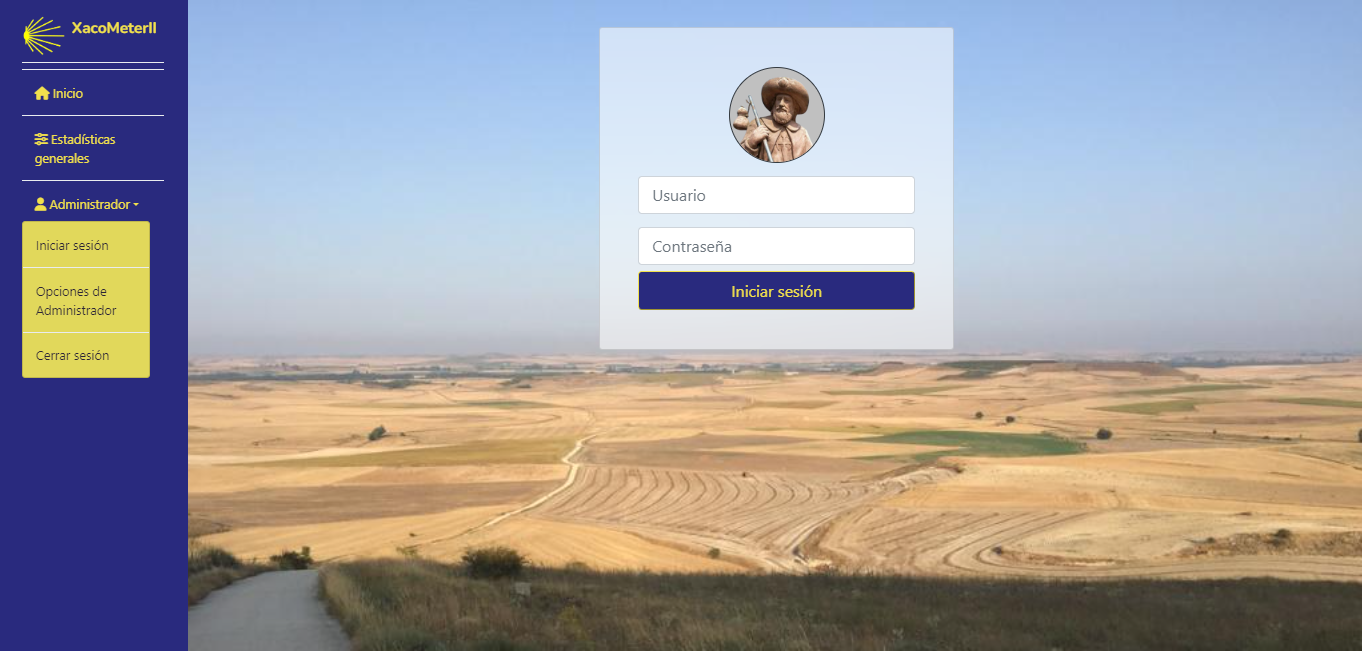
\includegraphics[scale=0.3]{img/Login.png} \\
    \caption{Documentación de usuario - Inicio de sesión}
    \label{Documentación de usuario - Inicio de sesión}
\end{figure}

\subsection{Opciones del administrador}
El administrador tiene tres opciones (Figura E.17):
\begin{enumerate}
    \item Crear una base de datos desde una fecha.
    \item Actualizar la base de datos desde la última fecha registrada hasta el día de hoy.
    \item Cerrar la sesión.
\end{enumerate}
Para acceder a cualquiera de estas tres opciones, se debe seleccionar sobre uno de los botones de esta página.
\begin{figure}[h!]
    \centering
    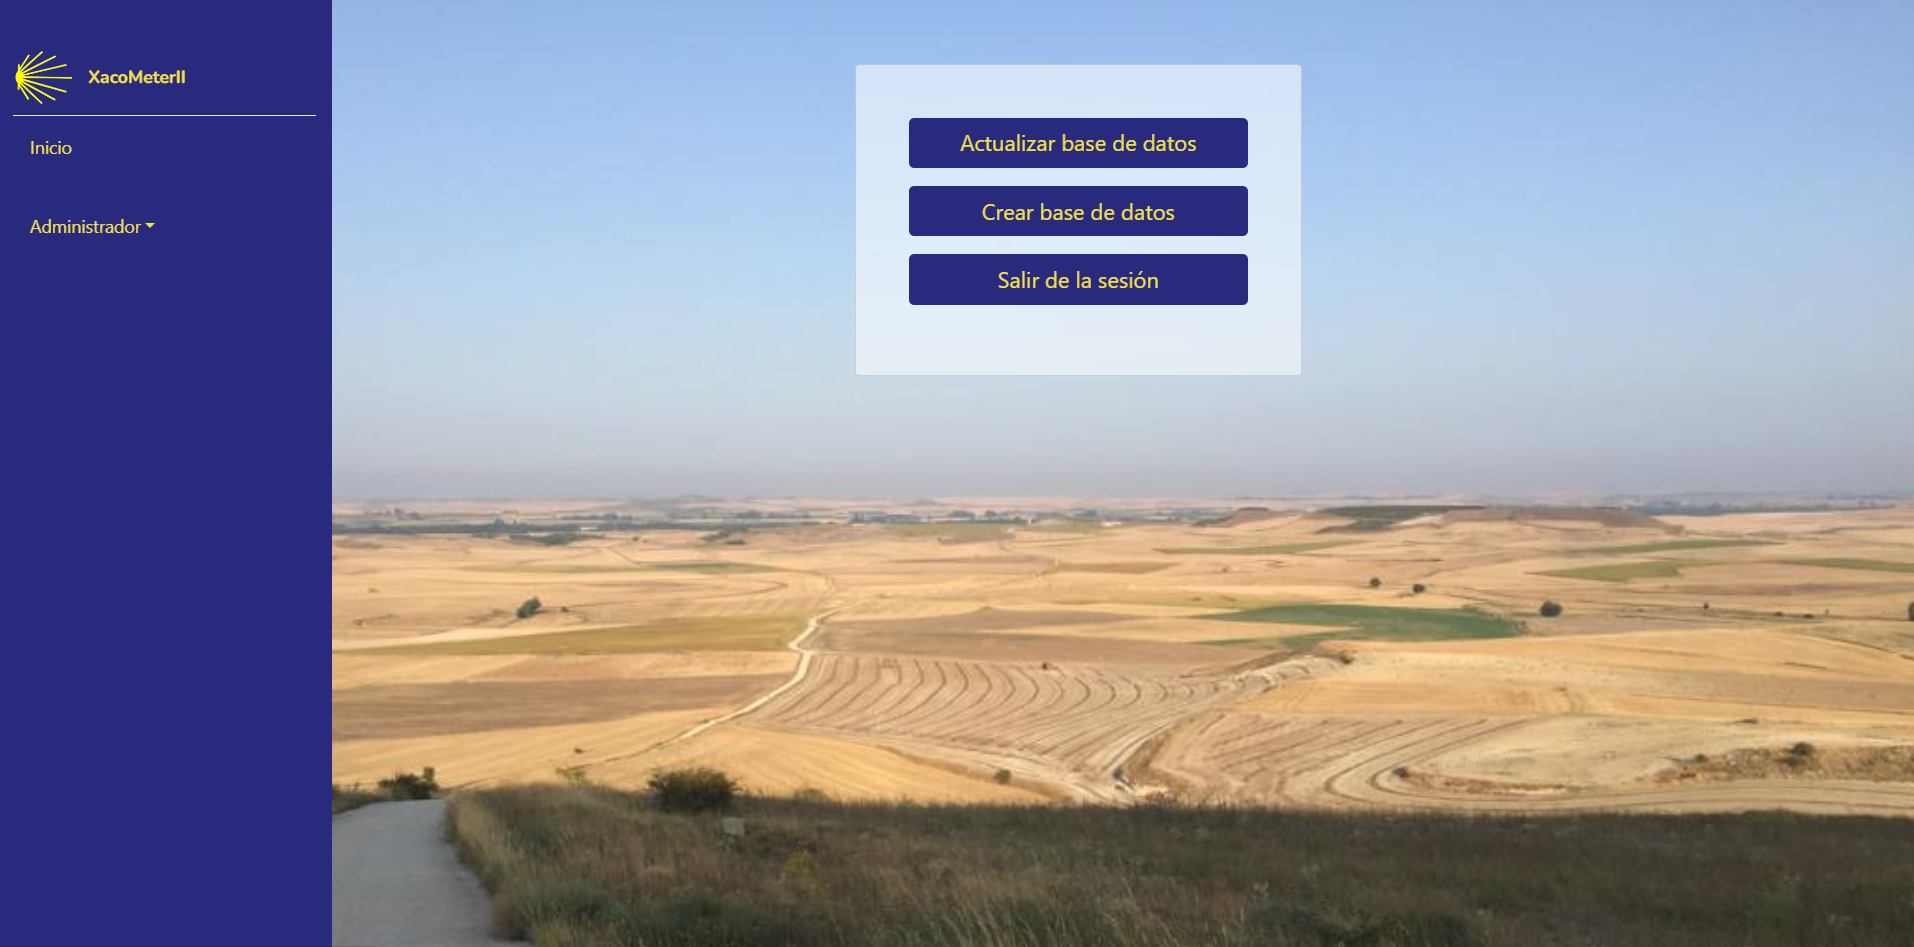
\includegraphics[scale=0.2]{img/OpcionesAdministrador.png} \\
    \caption{Documentación de usuario - Opciones del administrador}
    \label{Documentación de usuario - Opciones del administrador}
\end{figure}
\subsubsection{Creación de la base de datos}
En el caso de ser administrador y querer crear una base de datos, se requerirán unos parámetros para realizar las búsquedas (Figura E.18). Estos son las fechas que se quieren consultar y otros parámetros establecidos por Twitter que limitan nuestra búsqueda:
\begin{enumerate}
     \item Introducir las consultas que se van a realizar. Actualmente solo se pueden realizar máximo 300 consultas cada 15 minutos.
    \item El tiempo de duración de cada petición. Actualmente cada petición debe durar mínimo 1 segundo.
    \item El tiempo de espera entre las consultas especificadas en el primer parámetro y las siguientes consultas. Twitter ha definido que se podrán realizar máximo 300 consultas cada 15 minutos, por lo que se recomienda esperar 10 minutos, es decir, 600 segundos:\\
    $$ 15\hspace{0.5em}minutos\times60\frac{\text{segundos}}{\text{minuto}}=900\hspace{0.5em}segundos $$
    $$ 300\hspace{0.5em}peticiones\times1\frac{\text{segundo}}{\text{petición}}=300\hspace{0.5em}segundos $$
    $$ 900\hspace{0.5em}segundos\hspace{0.5em}-\hspace{0.5em} 300\hspace{0.5em}segundos\hspace{0.5em}=\hspace{0.5em}600\hspace{0.5em}segundos$$
\end{enumerate}
\begin{figure}[h!]
    \centering
    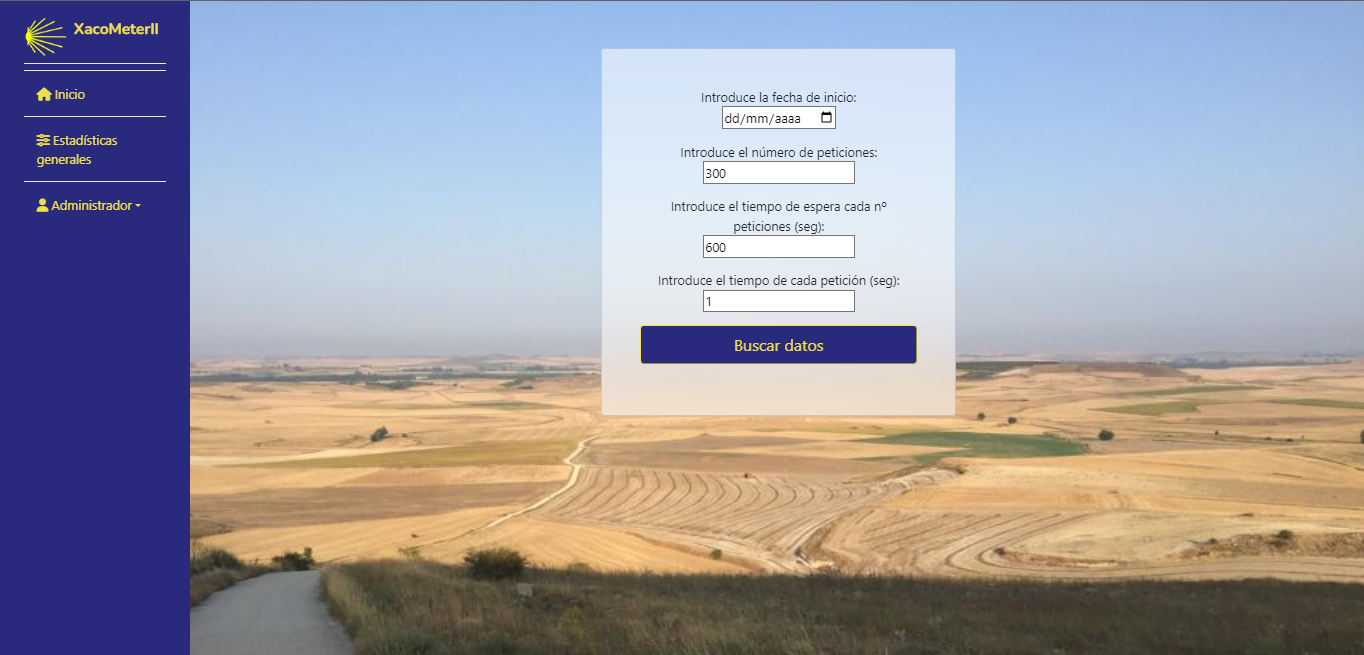
\includegraphics[scale=0.4]{img/CrearBD.png} \\
    \caption{Documentación de usuario - Crear base de datos}
    \label{Documentación de usuario - Crear base de datos}
\end{figure}
\subsection{Actualización de la base de datos}
Al igual que en el caso de 'Creación de la base de datos', se puede actualizar la base de datos marcando la fecha automáticamente, dándole el último valor de fecha almacenado en la base de datos. El usuario debe introducir los parámetros en base a las restricciones de Twitter (Figura E.19):\\
\begin{enumerate}
     \item Introducir las consultas que se van a realizar. Actualmente solo se podrán realizar máximo 300 consultas cada 15 minutos.
    \item El tiempo de duración de cada petición. Actualmente cada petición debe durar mínimo 1 segundo.
    \item El tiempo de espera entre las consultas especificadas en el primer parámetro y las siguientes consultas. Twitter ha definido que se podrán realizar máximo 300 consultas cada 15 minutos, por lo que se recomienda esperar 10 minutos, es decir, 600 segundos:\\
    $$ 15\hspace{0.5em}minutos\times60\frac{\text{segundos}}{\text{minuto}}=900\hspace{0.5em}segundos $$
    $$ 300\hspace{0.5em}peticiones\times1\frac{\text{segundo}}{\text{petición}}=300\hspace{0.5em}segundos $$
    $$ 900\hspace{0.5em}segundos\hspace{0.5em}-\hspace{0.5em} 300\hspace{0.5em}segundos\hspace{0.5em}=\hspace{0.5em}600\hspace{0.5em}segundos$$
\end{enumerate}
\begin{figure}[h!]
    \centering
    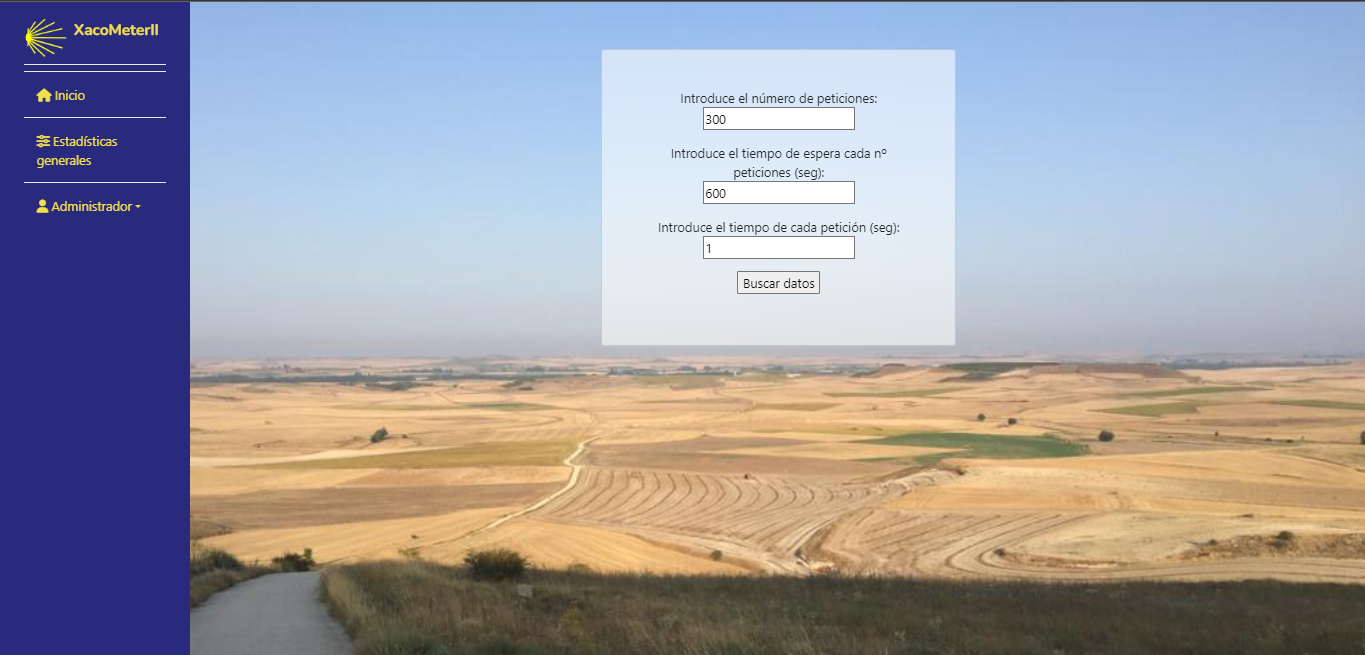
\includegraphics[scale=0.4]{img/ActualizarBD.png} \\
    \caption{Documentación de usuario - Actualizar base de datos}
    \label{Documentación de usuario - Actualizar base de datos}
\end{figure}
\subsection{Cerrar sesión}
En el caso de estar iniciada la sesión de 'Administrador', se puede salir de la sesión pulsando el botón \textbf{'Cerrar sesión'} (Figura E.20).\\
La sesión dura abierta 30 minutos, por lo que en el caso de querer continuar en la sesión se requerirá volver a introducir las credenciales.
\begin{figure}[h!]
    \centering
    
\includegraphics[scale=0.75]{img/CerrarSesion.png} \\
    \caption{Documentación de usuario - Cierre de sesión}
    \label{Documentación de usuario - Cierre de sesión}
\end{figure}

